% Created by tikzDevice version 0.12
% !TEX encoding = UTF-8 Unicode
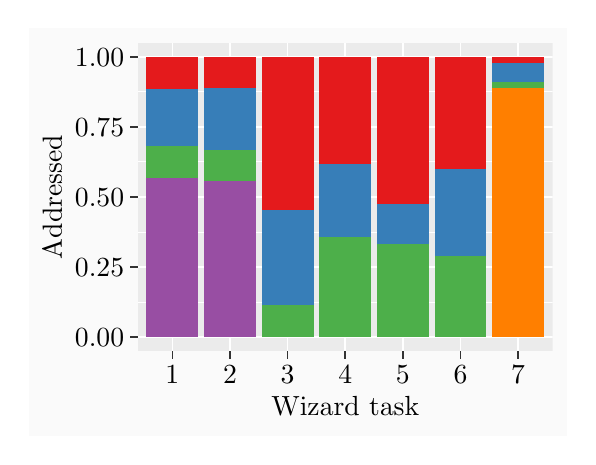
\begin{tikzpicture}[x=1pt,y=1pt]
\definecolor{fillColor}{RGB}{255,255,255}
\path[use as bounding box,fill=fillColor,fill opacity=0.00] (0,0) rectangle (195.19,147.70);
\begin{scope}
\path[clip] (  0.00,  0.00) rectangle (195.19,147.70);
\definecolor{drawColor}{RGB}{255,255,255}
\definecolor{fillColor}{gray}{0.98}

\path[draw=drawColor,line width= 0.6pt,line join=round,line cap=round,fill=fillColor] (  0.00,  0.00) rectangle (195.19,147.70);
\end{scope}
\begin{scope}
\path[clip] ( 39.80, 30.86) rectangle (189.69,142.20);
\definecolor{fillColor}{gray}{0.92}

\path[fill=fillColor] ( 39.80, 30.86) rectangle (189.69,142.20);
\definecolor{drawColor}{RGB}{255,255,255}

\path[draw=drawColor,line width= 0.3pt,line join=round] ( 39.80, 48.58) --
	(189.69, 48.58);

\path[draw=drawColor,line width= 0.3pt,line join=round] ( 39.80, 73.88) --
	(189.69, 73.88);

\path[draw=drawColor,line width= 0.3pt,line join=round] ( 39.80, 99.19) --
	(189.69, 99.19);

\path[draw=drawColor,line width= 0.3pt,line join=round] ( 39.80,124.49) --
	(189.69,124.49);

\path[draw=drawColor,line width= 0.6pt,line join=round] ( 39.80, 35.92) --
	(189.69, 35.92);

\path[draw=drawColor,line width= 0.6pt,line join=round] ( 39.80, 61.23) --
	(189.69, 61.23);

\path[draw=drawColor,line width= 0.6pt,line join=round] ( 39.80, 86.53) --
	(189.69, 86.53);

\path[draw=drawColor,line width= 0.6pt,line join=round] ( 39.80,111.84) --
	(189.69,111.84);

\path[draw=drawColor,line width= 0.6pt,line join=round] ( 39.80,137.14) --
	(189.69,137.14);

\path[draw=drawColor,line width= 0.6pt,line join=round] ( 52.29, 30.86) --
	( 52.29,142.20);

\path[draw=drawColor,line width= 0.6pt,line join=round] ( 73.11, 30.86) --
	( 73.11,142.20);

\path[draw=drawColor,line width= 0.6pt,line join=round] ( 93.93, 30.86) --
	( 93.93,142.20);

\path[draw=drawColor,line width= 0.6pt,line join=round] (114.75, 30.86) --
	(114.75,142.20);

\path[draw=drawColor,line width= 0.6pt,line join=round] (135.56, 30.86) --
	(135.56,142.20);

\path[draw=drawColor,line width= 0.6pt,line join=round] (156.38, 30.86) --
	(156.38,142.20);

\path[draw=drawColor,line width= 0.6pt,line join=round] (177.20, 30.86) --
	(177.20,142.20);
\definecolor{fillColor}{RGB}{152,78,163}

\path[fill=fillColor] ( 42.93, 35.92) rectangle ( 61.66, 93.43);
\definecolor{fillColor}{RGB}{77,175,74}

\path[fill=fillColor] ( 42.93, 93.43) rectangle ( 61.66,104.94);
\definecolor{fillColor}{RGB}{55,126,184}

\path[fill=fillColor] ( 42.93,104.94) rectangle ( 61.66,125.64);
\definecolor{fillColor}{RGB}{228,26,28}

\path[fill=fillColor] ( 42.93,125.64) rectangle ( 61.66,137.14);
\definecolor{fillColor}{RGB}{152,78,163}

\path[fill=fillColor] ( 63.74, 35.92) rectangle ( 82.48, 92.16);
\definecolor{fillColor}{RGB}{77,175,74}

\path[fill=fillColor] ( 63.74, 92.16) rectangle ( 82.48,103.40);
\definecolor{fillColor}{RGB}{55,126,184}

\path[fill=fillColor] ( 63.74,103.40) rectangle ( 82.48,125.90);
\definecolor{fillColor}{RGB}{228,26,28}

\path[fill=fillColor] ( 63.74,125.90) rectangle ( 82.48,137.14);
\definecolor{fillColor}{RGB}{77,175,74}

\path[fill=fillColor] ( 84.56, 35.92) rectangle (103.30, 47.43);
\definecolor{fillColor}{RGB}{55,126,184}

\path[fill=fillColor] ( 84.56, 47.43) rectangle (103.30, 81.93);
\definecolor{fillColor}{RGB}{228,26,28}

\path[fill=fillColor] ( 84.56, 81.93) rectangle (103.30,137.14);
\definecolor{fillColor}{RGB}{77,175,74}

\path[fill=fillColor] (105.38, 35.92) rectangle (124.11, 72.07);
\definecolor{fillColor}{RGB}{55,126,184}

\path[fill=fillColor] (105.38, 72.07) rectangle (124.11, 98.58);
\definecolor{fillColor}{RGB}{228,26,28}

\path[fill=fillColor] (105.38, 98.58) rectangle (124.11,137.14);
\definecolor{fillColor}{RGB}{77,175,74}

\path[fill=fillColor] (126.19, 35.92) rectangle (144.93, 69.66);
\definecolor{fillColor}{RGB}{55,126,184}

\path[fill=fillColor] (126.19, 69.66) rectangle (144.93, 84.12);
\definecolor{fillColor}{RGB}{228,26,28}

\path[fill=fillColor] (126.19, 84.12) rectangle (144.93,137.14);
\definecolor{fillColor}{RGB}{77,175,74}

\path[fill=fillColor] (147.01, 35.92) rectangle (165.75, 65.16);
\definecolor{fillColor}{RGB}{55,126,184}

\path[fill=fillColor] (147.01, 65.16) rectangle (165.75, 96.66);
\definecolor{fillColor}{RGB}{228,26,28}

\path[fill=fillColor] (147.01, 96.66) rectangle (165.75,137.14);
\definecolor{fillColor}{RGB}{255,127,0}

\path[fill=fillColor] (167.83, 35.92) rectangle (186.56,125.90);
\definecolor{fillColor}{RGB}{77,175,74}

\path[fill=fillColor] (167.83,125.90) rectangle (186.56,128.15);
\definecolor{fillColor}{RGB}{55,126,184}

\path[fill=fillColor] (167.83,128.15) rectangle (186.56,134.89);
\definecolor{fillColor}{RGB}{228,26,28}

\path[fill=fillColor] (167.83,134.89) rectangle (186.56,137.14);
\end{scope}
\begin{scope}
\path[clip] (  0.00,  0.00) rectangle (195.19,147.70);
\definecolor{drawColor}{RGB}{0,0,0}

\node[text=drawColor,anchor=base east,inner sep=0pt, outer sep=0pt, scale=  1.00] at ( 34.85, 32.48) {0.00};

\node[text=drawColor,anchor=base east,inner sep=0pt, outer sep=0pt, scale=  1.00] at ( 34.85, 57.78) {0.25};

\node[text=drawColor,anchor=base east,inner sep=0pt, outer sep=0pt, scale=  1.00] at ( 34.85, 83.09) {0.50};

\node[text=drawColor,anchor=base east,inner sep=0pt, outer sep=0pt, scale=  1.00] at ( 34.85,108.39) {0.75};

\node[text=drawColor,anchor=base east,inner sep=0pt, outer sep=0pt, scale=  1.00] at ( 34.85,133.70) {1.00};
\end{scope}
\begin{scope}
\path[clip] (  0.00,  0.00) rectangle (195.19,147.70);
\definecolor{drawColor}{gray}{0.20}

\path[draw=drawColor,line width= 0.6pt,line join=round] ( 37.05, 35.92) --
	( 39.80, 35.92);

\path[draw=drawColor,line width= 0.6pt,line join=round] ( 37.05, 61.23) --
	( 39.80, 61.23);

\path[draw=drawColor,line width= 0.6pt,line join=round] ( 37.05, 86.53) --
	( 39.80, 86.53);

\path[draw=drawColor,line width= 0.6pt,line join=round] ( 37.05,111.84) --
	( 39.80,111.84);

\path[draw=drawColor,line width= 0.6pt,line join=round] ( 37.05,137.14) --
	( 39.80,137.14);
\end{scope}
\begin{scope}
\path[clip] (  0.00,  0.00) rectangle (195.19,147.70);
\definecolor{drawColor}{gray}{0.20}

\path[draw=drawColor,line width= 0.6pt,line join=round] ( 52.29, 28.11) --
	( 52.29, 30.86);

\path[draw=drawColor,line width= 0.6pt,line join=round] ( 73.11, 28.11) --
	( 73.11, 30.86);

\path[draw=drawColor,line width= 0.6pt,line join=round] ( 93.93, 28.11) --
	( 93.93, 30.86);

\path[draw=drawColor,line width= 0.6pt,line join=round] (114.75, 28.11) --
	(114.75, 30.86);

\path[draw=drawColor,line width= 0.6pt,line join=round] (135.56, 28.11) --
	(135.56, 30.86);

\path[draw=drawColor,line width= 0.6pt,line join=round] (156.38, 28.11) --
	(156.38, 30.86);

\path[draw=drawColor,line width= 0.6pt,line join=round] (177.20, 28.11) --
	(177.20, 30.86);
\end{scope}
\begin{scope}
\path[clip] (  0.00,  0.00) rectangle (195.19,147.70);
\definecolor{drawColor}{RGB}{0,0,0}

\node[text=drawColor,anchor=base,inner sep=0pt, outer sep=0pt, scale=  1.00] at ( 52.29, 19.03) {1};

\node[text=drawColor,anchor=base,inner sep=0pt, outer sep=0pt, scale=  1.00] at ( 73.11, 19.03) {2};

\node[text=drawColor,anchor=base,inner sep=0pt, outer sep=0pt, scale=  1.00] at ( 93.93, 19.03) {3};

\node[text=drawColor,anchor=base,inner sep=0pt, outer sep=0pt, scale=  1.00] at (114.75, 19.03) {4};

\node[text=drawColor,anchor=base,inner sep=0pt, outer sep=0pt, scale=  1.00] at (135.56, 19.03) {5};

\node[text=drawColor,anchor=base,inner sep=0pt, outer sep=0pt, scale=  1.00] at (156.38, 19.03) {6};

\node[text=drawColor,anchor=base,inner sep=0pt, outer sep=0pt, scale=  1.00] at (177.20, 19.03) {7};
\end{scope}
\begin{scope}
\path[clip] (  0.00,  0.00) rectangle (195.19,147.70);
\definecolor{drawColor}{RGB}{0,0,0}

\node[text=drawColor,anchor=base,inner sep=0pt, outer sep=0pt, scale=  1.00] at (114.75,  7.44) {Wizard task};
\end{scope}
\begin{scope}
\path[clip] (  0.00,  0.00) rectangle (195.19,147.70);
\definecolor{drawColor}{RGB}{0,0,0}

\node[text=drawColor,rotate= 90.00,anchor=base,inner sep=0pt, outer sep=0pt, scale=  1.00] at ( 12.39, 86.53) {Addressed};
\end{scope}
\end{tikzpicture}
